\chapter{Young Entrepreneur Interviews Patrick Bet-David}

This interview from School of Hard Knocks, curated here by LazyingArt LLC, is not a lecture in the usual classroom sense, but it does have a clean mathematical backbone. Numbers keep appearing at the points where the argument tightens: annual revenue, agent counts, failure rates, employees, CEOs, purchase prices, deposits, valuations, years of delay, and simple if-then rules about focus, cash, attention, and desperation. The safest way to write the chapter is to let the logic unfold in the same order as the transcript: first the teaser of scale, then the discipline of concentration, then the operator, then the larger framework of growth, then liquidity, then media fit, then sales and valuation, and only at the end the philosophy of money and belief.

\section{Cold Open: Scale Before Explanation}

The lecture begins by showing us the later peaks before it tells us how they were produced. We are given, in compressed form, a very large annual revenue number, a mansion auction narrated through a funnel of hard counts, and a terse thesis about cash. This is not yet the argument. It is a trailer for the argument.

The opening arithmetic is deliberately memorable:
\begin{align}
Y_{\max} &= \$250\,\text{million},\\
N_{\text{interest}} &= 4400,\qquad N_{\text{NDA}} = 131,\qquad D_{\text{bid}} = \$1\,\text{million},\\
P_{\text{buy}} &= \$25.2\,\text{million cash}.
\end{align}
The important point is not merely that the numbers are large. It is that the lecture begins with consequence and only later turns to cause. We are meant to ask what kind of machine makes these later outcomes possible.

After the cold open, the host resets the scene in Miami and promises a masterclass on business, sales, negotiation, and money. Then, before the doctrine begins, there is a short motivational prelude. Bet-David praises the host's age, reach, and seriousness. This matters because the lecture wants to frame attention itself as leverage before it turns to insurance, management, and scale.

\section{Concentration Before Diversification}

The first real doctrine arrives through industry choice. Bet-David says he first built wealth in insurance and only later expanded into media and consulting. He then gives the lecture's first slogan: concentration builds wealth; diversification keeps it. The point is not merely rhetorical. It is a statement about organizational dynamics. A business compounds more cleanly when it is not trying to do too many adjacent things at once.

His threshold for diversification is intentionally rough:
\begin{equation}
W_{\text{diversify}} \gtrsim \$10\,\text{billion}.
\end{equation}
The transcript does not tell us exactly what this threshold measures, so the final notes should keep it approximate and speaker-attributed.

The supporting mechanism comes through the Blue Ocean story. He recalls entering insurance, reading \emph{Blue Ocean Strategy}, calling an emergency meeting, and then cutting away disability, stocks, bonds, mutual funds, variable annuities, and the rest of the surrounding sprawl. The transcript contains a garbled line about licenses, but the usable point is straightforward: he concentrated on life insurance and stopped diffusing the machine.

The numerical evidence is the simplest and strongest in the section:
\begin{equation}
N_{\text{agents}} : 66 \longrightarrow 60{,}000.
\end{equation}
This is the lecture's first proof by scale. Focus is not being defended as a mood or aesthetic. It is being defended by what happened after the product set was narrowed.

\subsection{Question \& Answer}

\paragraph{Question.} Why does narrowing the business create scale rather than limit it?

\paragraph{Answer.} Because narrowing removes internal friction. Training, sales language, recruiting, and repetition all begin to point in one direction. The organization stops paying the tax of variety. In the speaker's logic, diversification is not denied forever; it is postponed until the core machine has already compounded.

\section{The Operator: Focus, Stability, and Cultural Filtering}

The lecture now moves from the business model to the person running it. The host asks why so many companies fail. Bet-David answers by relocating the cause from the market to the operator. The introduced heuristic is:
\begin{equation}
p_{\text{fail},5\text{yr}} \approx \frac{8}{10}.
\end{equation}
Whatever the exact external validity of that number, the lecture uses it to motivate a stricter causal claim: everything rises and falls on the operator.

A compact notation for the speaker's bundle of concerns is
\begin{equation}
\mathcal{O}=\{\text{focus},\ \text{emotional stability},\ \text{feedback judgment}\}.
\end{equation}
The point is not to pretend these variables were measured. The point is that they function as the hidden state of the company. If the operator is distracted, unstable, or unable to distinguish useful feedback from prestigious but harmful feedback, the organization loses coherence.

This is where the lecture's cultural argument sharpens. Bet-David gives the example of hiring someone with a Harvard degree and then allowing the degree itself to rewrite the company's culture. The danger is not learning. The danger is surrendering directional judgment.

We can therefore write the section's governing implication as
\begin{equation}
\text{operator weakness} \Rightarrow \text{scaling difficulty}.
\end{equation}
The lecture is careful here. It is not saying that every difficulty is psychological. It is saying that strategy by itself is not enough if the operating center is unstable.

\subsection{Question \& Answer}

\paragraph{Question.} How do we take feedback without letting outside prestige dissolve the company's culture?

\paragraph{Answer.} By filtering feedback through mission and fit rather than through status. The lecture does not dismiss degrees; it dismisses passive deference. Advice is useful only if it strengthens the machine we are actually trying to build.

\section{A Commercial Interruption, Then the CEO Problem}

At this point the video pauses for the host's School of Mentors promotion. In the transcript this is not accidental noise; it is part of the pacing. The line of argument breaks, the host sells mentorship through his network, and then the interview restarts. The best notes should preserve that restart rather than pretending the lecture moved forward continuously.

When the conversation resumes, the new question is sharper than the earlier one: what took the company from eight to nine figures? Bet-David answers first by admitting a limit. Around
\begin{equation}
Y \approx \$10\,\text{million/year},
\end{equation}
he thought of himself as a strong sales leader and a disciplined steward of money, but not yet a real operator. That confession matters, because it creates the need for the lecture's strongest conceptual apparatus.

The answer comes through Harvard OPM:
\begin{equation}
N_{\text{CEO}}=144,\qquad N_{\text{countries}}=64.
\end{equation}
There he meets a much larger operator, described as the Victoria's Secret analogue for New Zealand and Australia, with the stated scale
\begin{equation}
W_{\text{peer}} \approx \$1.5\,\text{billion},\qquad
N_{\text{employees}}=7000,\qquad
N_{\text{CEO reports}}=6.
\end{equation}
The peer then gives the lecture's most important framework. Since no validated board image survives, we reconstruct the structure cautiously from the spoken order:
\begin{equation}
G_{\text{linear}}=\{\text{biz dev},\ \text{systems}\},\qquad
G_{\text{exp}}=\{\text{leadership development},\ \text{innovative campaigns}\}.
\end{equation}
The implied hierarchy is
\begin{equation}
G_{\text{exp}} > G_{\text{linear}}
\qquad\text{for explosive upside.}
\end{equation}
The lecture does not mean that business development, systems, and networking are dispensable. It means that they typically extend the present machine, whereas leadership development and original campaigns can alter the machine's scale law.

\begin{figure}[h]
\centering
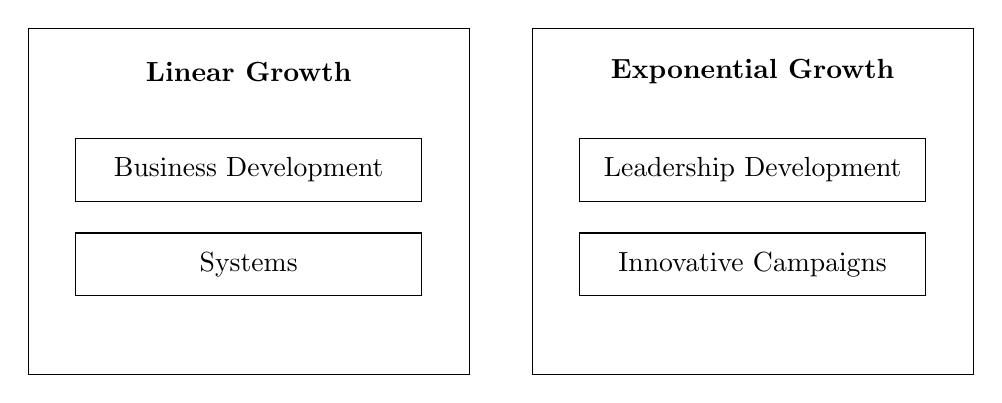
\begin{tikzpicture}
\draw (0,0) rectangle (5.6,4.4);
\draw (6.4,0) rectangle (12.0,4.4);

\node at (2.8,3.85) {\textbf{Linear Growth}};
\node at (9.2,3.85) {\textbf{Exponential Growth}};

\draw (0.6,3.0) rectangle (5.0,2.2);
\draw (0.6,1.8) rectangle (5.0,1.0);

\draw (7.0,3.0) rectangle (11.4,2.2);
\draw (7.0,1.8) rectangle (11.4,1.0);

\node at (2.8,2.6) {Business Development};
\node at (2.8,1.4) {Systems};

\node at (9.2,2.6) {Leadership Development};
\node at (9.2,1.4) {Innovative Campaigns};
\end{tikzpicture}
\caption{A cautious transcript-led reconstruction of the four growth levers introduced in the Harvard OPM story.}
\end{figure}

The Coke example, ``share a Coke with John,'' shows what the lecture means by innovation. The point is not technological novelty. The point is a campaign that changes who buys, why they buy, and how the brand enters social circulation.

\subsection{Question \& Answer}

\paragraph{Question.} Why do systems and business development help a company grow without necessarily making it explode?

\paragraph{Answer.} Because they improve the reach and efficiency of the current machine without changing its regime. Systems reduce waste. Business development extends current processes. Leadership development and strong campaigns can instead change the structure of execution or the market's perception of the offer, and therefore produce discontinuous jumps.

\section{Cash as Optionality}

Having built a framework for growth, the lecture pivots into treasury. Asked for the best financial advice he ever received, Bet-David answers: always have cash. This is not offered as a conservative slogan. It is offered as a rule about optionality under stress.

The Wayne Gretzky card story is the first clean example:
\begin{align}
P_0 &= \$540{,}000,\\
V_{1.5\text{ yr}} &= \$2.2\,\text{million},\\
\frac{V_{1.5\text{ yr}}}{P_0} &\approx 4.07.
\end{align}
The lecture is not really about collectibles. The underlying mechanism is timing. A seller has immediate need; a buyer with available cash can compress the transaction window and harvest the mismatch.

The same pattern returns at a larger scale in real estate:
\begin{align}
P_{2018} &= \$25\,\text{million},\qquad
C_{\text{finish}} = \$7\,\text{million},\\
N_{\text{interest}} &= 4400,\qquad
N_{\text{NDA}} = 131,\qquad
D_{\text{bid}} = \$1\,\text{million},\\
P_{\text{buy}} &= \$25.2\,\text{million cash},\qquad
V_{\text{est}} \approx \$40\text{--}50\,\text{million}.
\end{align}
A small worked example clarifies the logic. Relative to the previous owner's stated basis,
\begin{align}
B_{\text{old}} &= P_{2018}+C_{\text{finish}} = 25+7 = \$32\,\text{million},\\
B_{\text{old}}-P_{\text{buy}} &= 32-25.2 = \$6.8\,\text{million}.
\end{align}
Relative to the speaker's own rough estimate of current value, the implied gap is
\begin{align}
\Delta V_{\text{low}} &= 40-25.2 = \$14.8\,\text{million},\\
\Delta V_{\text{high}} &= 50-25.2 = \$24.8\,\text{million}.
\end{align}
These later values are estimates, not audited appraisals, and they should remain labeled as such. But the logic is strong enough: stressed conditions plus ready cash can create access to assets below later perceived value.

The section's main rule is therefore
\begin{equation}
C_{\text{available}}+\text{market stress}\Rightarrow \text{mispricing access}.
\end{equation}
What looks like idle liquidity is, in this lecture, a stored option on future distress.

\section{The Market Tests the Message}

The lecture then leaves treasury and enters media through a sharp contrast: great businessmen are often poor content creators, and great content creators are often poor businessmen. Bet-David's answer is that the market decides whether communication works. The sentence is rough in the transcript, but the structure is crisp: attention is not granted by self-description.

The numbers of the early YouTube experiment matter:
\begin{equation}
t_{\text{early}} \approx 2\,\text{years},\qquad
N_{\text{subscribers}} \approx 1000.
\end{equation}
This is the lecture's brutal media premise. For about two years, the channel existed, but the market had not ratified it.

The adjustment was not generic persistence. It was narrowing. He was told to pick one word, and the word became business and entrepreneurship. Then the titles became disciplined variations on that niche. The later result is summarized as
\begin{equation}
s_{\text{page1}} \approx 50\%.
\end{equation}
The lecture treats this not as vanity, but as evidence that the message had found its search space.

This gives us a second market rule:
\begin{equation}
\text{market response}\Rightarrow \text{proof or refutation of message fit}.
\end{equation}
And the lecture pairs that rule with a heuristic communication taxonomy:
\begin{equation}
\mathcal{M}=\{\text{speaking},\ \text{video},\ \text{writing}\}.
\end{equation}
The point is not that everyone excels in all three. The point is that message must find both a medium and a market.

\subsection{Question \& Answer}

\paragraph{Question.} What does it mean for the market to tell us whether our message actually works?

\paragraph{Answer.} It means that our own belief in our clarity is irrelevant until attention confirms it. The lecture treats poor early performance as feedback, not as fate. Niche refinement, title discipline, and repeated testing are then ways of turning the market from a judge into a teacher.

\section{Needs Analysis, Desperation, and Valuation}

From media the lecture returns to the problem of persuasion. Bet-David's sales doctrine is needs analysis. We are to ask what matters to the other side before deciding what to recommend. His examples begin at home, with children whose preferences differ from parental projections, and then move back to clients. That order is useful. The lecture domesticates the mechanism before generalizing it.

A compact formalization is
\begin{equation}
R^*=\arg\max_R \operatorname{Fit}(R,\text{buyer priorities}).
\end{equation}
A recommendation chosen before the buyer's priorities are known is merely the seller replaying his favorite script.

That same commitment to structure rather than impulse carries into negotiation:
\begin{equation}
\text{desperation}\Rightarrow \text{underpricing}+\text{bad decisions}.
\end{equation}
The company-sale story is the lecture's cleanest proof. A first buyer offers
\begin{equation}
V_1=\$120\,\text{million},\qquad
U_1=50\%\ \text{upfront},\qquad
T_{\text{stay}}=5\,\text{years}.
\end{equation}
The reason is revealing. Employees tell the buyer that Bet-David is the hardest-working person in the company. What looks admirable to an insider looks risky to an acquirer. In effect, the firm appears to be founder exertion disguised as enterprise.

The lecture's corresponding valuation rule is
\begin{equation}
\text{founder-centric operation}\Rightarrow \text{valuation discount}.
\end{equation}
The response is not to negotiate harder. It is to redesign the object being sold. He moves to Florida, hires
\begin{equation}
N_{\text{new C-suite}}=5
\end{equation}
new executives, reduces his own operational centrality, and waits
\begin{equation}
t_{\text{wait}}=2\,\text{years}.
\end{equation}
When the next buyer comes through, the company no longer sounds like one man working seven days a week. It sounds like an organization.

The transcript's payoff is striking:
\begin{align}
V_2 &> 2V_1,\\
V_2 &> 2\times \$120\,\text{million} = \$240\,\text{million}.
\end{align}
This lower bound is worth keeping in the notes. It lets us see in one line what the lecture is really claiming: architecture can change price more than effort can.

\subsection{Question \& Answer}

\paragraph{Question.} Why can removing the founder from daily operations increase valuation more than simply working harder inside the company?

\paragraph{Answer.} Because an acquirer buys transferable structure. If the company's earnings are inseparable from one person's presence, the buyer is buying fragility. Once leadership is distributed and repeatable, the company becomes legible as an asset in its own right, and valuation changes accordingly.

\section{Belief, Money, and Access}

Only after the lecture has moved through concentration, operator quality, growth, liquidity, media, sales, and valuation does it widen into philosophy. The host asks what separates middle-class thinking from long-term wealth building. Bet-David's answer is not a balance-sheet formula. It is a doctrine of refusal: do not inherit beliefs about money, marriage, class, or possibility merely because they came from family or circumstance.

This final movement is easy to flatten into generic uplift, but it is more precise than that. The earlier sections repeatedly taught the same lesson in commercial form. We do not accept diversification by default; we test concentration. We do not accept prestige by default; we test feedback. We do not accept a message by default; we test market response. The closing simply lifts that same discipline into the domain of belief.

The final doctrinal compression is therefore
\begin{equation}
\text{access to information}\Rightarrow \text{capacity for life change}.
\end{equation}
This is not a theorem in any strong sense. It is the lecture's closing heuristic. Its function is to deny the inevitability of excuse-structures in a world where information is far more widely distributed than it once was.

\section{Summary}

The lecture begins with scale and ends with philosophy, but the route between those two poles is orderly. First we are shown later outcomes. Then we are told that concentration makes compounding possible. Then we are told that the operator determines whether focus can be sustained. Then a larger operator provides a framework for thinking about linear and exponential growth. From there the lecture turns to cash, which is recast as optionality; then to media, where the market tests the message; then to sales and negotiation, where needs analysis and non-desperation protect price; and finally to belief, where inherited limits are placed under criticism.

The chain of implications may be written compactly as
\begin{align}
\text{concentration} &\Rightarrow \text{compounding focus},\\
\text{operator quality} &\Rightarrow \text{organizational durability},\\
\text{cash} &\Rightarrow \text{optionality under stress},\\
\text{message-market fit} &\Rightarrow \text{media scale},\\
\text{founder decoupling} &\Rightarrow \text{higher valuation},\\
\text{belief revision} &\Rightarrow \text{commercial revision}.
\end{align}
That is the lecture's real architecture. The spectacular numbers at the beginning are not the content of the lecture. They are the shadows cast by structure: by focus, by operating discipline, by liquidity, by message fit, by company design, and by a refusal to let inherited beliefs govern what can be built.